
%% Template by Michal Forisek


\documentclass[a4paper]{report}
\usepackage{slovak}
\usepackage[utf8]{inputenc}
\usepackage{a4wide}
\usepackage{tabularx}
\usepackage{amsfonts}
\usepackage{amssymb}
\usepackage{amsmath}
\usepackage{epsfig}
\usepackage{color}
\usepackage{mathrsfs}
\usepackage{verbatim}
\usepackage{hyperref}
\usepackage{algorithm2e}


\def\todo#1{[{\color{red} TODO:} {\bf  #1}]}
\def\fixme#1{[{\color{red} FIXME:} {\bf  #1}]}
\def\verify#1{\todo{verify: #1}}

\renewcommand{\implies}{\rightarrow}
\newcommand{\notmodels}{\nvDash}
\newcommand{\union}{\cup}
\newcommand{\provable}{\vdash}
\newcommand{\unprovable}{\nvdash}

\def\noheader{\relax}

\newtheorem{definicia}{Definícia}[section]
\newtheorem{HLPpriklad}{Príklad}[section]
\newenvironment{priklad}[1][]{
    \ifthenelse{\equal{#1}{}}{
        \begin{HLPpriklad}
    }{
        \begin{HLPpriklad}[#1]
    }
    \rm}{\end{HLPpriklad}
}
\newtheorem{veta}{Veta}[section]
\newtheorem{lema}{Lema}[section]


\newenvironment{dokaz}{\trivlist
  \item[\hskip \labelsep{\bfseries Dôkaz:}]}{\endtrivlist}


\begin{document}

\thispagestyle{empty}
\begin{minipage}{0.25\textwidth}
\includegraphics[width=0.9\textwidth]{img/komlogo-new}
\end{minipage}
\begin{minipage}{0.69\textwidth}
\begin{center}
\sc Katedra Informatiky \\
Fakulta Matematiky, Fyziky a Informatiky \\
Univerzita Komenského, Bratislava
\end{center}
\end{minipage}

\vfill
\begin{center}
\begin{minipage}{0.8\textwidth}
\hrule
\bigskip\bigskip
\centerline{\LARGE\sc Krypto II}
\smallskip
\centerline{(spísané poznámky, draft)}
\bigskip
\bigskip
\centerline{\large\sc Vladimír Boža, Peter Perešíni}
\bigskip
\centerline{\large\sc (prednášal RNDr. Martin Stanek, PhD.)}
\bigskip\bigskip
\hrule
\end{minipage}
\end{center}
\vfill
{~}
\hfill verzia zo dňa {\bf\today} 
\eject % EOP i

\section*{Úvod a disclaimer}

Tieto poznámky obsahujú študijné materiály k predmetu 
\emph{Kryptológia II}
na Fakulte matematiky, fyziky a informatiky UK.
Základná verzia bola spísaná podľa prednášky RNDr. Martina Staneka v
roku 2010. Poznámky však nie sú oficiálny študijný materiál, preto
autori neručia za ich aktuálnosť a vhodnosť na štúdium. Navyše, obsah
prednášky sa môže z roka na rok meniť, a preto je odporúčané dávať
pozor na prípadné rozdiely a dopísať si časti nepokryté týmito
poznámkami.

Aby sme umožnoli jednoduchšie spravovanie a udržali poznámky dlhšie
aktuálne, rozhodli sme sa verejne publikovať zdrojové kódy na stránke
\url{http://code.google.com/p/krypto2}. Ak máte akékoľvek pripomienky,
návrhy, opravy, môžete nám ich prostredníctvom tejto stránky oznámiť.

PPershing a U\$ama.


\tableofcontents

\chapter{Úvod}
\label{chapter:uvod}
\section{Prerekvizity a označenia}

\todo{odkaz na skripta z krypto I}

V zvyšnom texte budeme dodržiavať (až na občasné výnimky) nasledujúce
označenia:
\begin{itemize}
\item $A,B$ - účastníci komunikácie, $E$ - útočník, $E(A)$ - útočník
            tváriaci sa ako účastník $A$.
\item $E(p,k), E_k(p)$ - zašifrovanie otvoreného textu $p$ pomocou kľúča $k$
\item $D(c,k), D_k(c)$ - odšifrovanie šifrového textu $c$ pomocou kľúča $k$
\item $E_A(m)$ - zašifrovanie správy $m$ pomocou verejného kľúča účastníka $A$
\item $D_A(c)$ - odšifrovanie správy $c$ pomocou súkromného kľúča účastníka $A$
\item $H(t)$ - spracovanie textu $t$ pomocou hashovacej funkcie $H$
\item $x \inr M$ - $x$ je \emph{náhodne zvolený} prvok množiny $M$
\item $\exists !$ - existuje práve jeden
\item $p(A)$ - pravdepodobnosť javu $A$
\item $p(A|B)$ - podmienená pravdepodobnosť, t.j. aká je pravdepodobnosť javu $A$, ak platí $B$
\end{itemize}

\section{0. prednáška - Ako (ne)šifrovať disky}

V decembri 2009 bola nájdená bezpečnostná chyba v niektorých šifrovaných USB diskoch
(Kingston DataTraveler BlackBox, SanDisk Cruzer Enterprise FIPS Edition a
Verbatim Corporate Secure FIPS Edition). Všetky výrobcovia uvádzajú, že disky
spĺňajú bezpečnostný štandart FIPS 140-2 a používajú úplne rovnaký systém zabezpečenia,
ktorý vyzerá nasledovne:
\begin{itemize}
\item Používateľ zadá disku heslo.
\item Heslo za pretransformuje cez MD5 hash a prvá polovica výslednej hashe sa použije ako kľúč K.
\item Následne sa pomocou AES-256 a kľúča K odšifruje daných 32 bajtov z disku (označme ich $X$). Potom zistí, či
$D_K(X)=C$, kde $C$ je pevne známa konštanta (u všetkých výrobcov dokonca rovnaká). Ak áno, tak sa disk odomkne a dáta sa sprístupnia.
Ak nie, tak sa požiadavka zamietne. Dešifrovanie ostatných dát nezávisí od hesla.
\end{itemize}

\begin{figure}[htp]
    \centering
    \includegraphics[scale=1]{img/00/extern-drive-encryption.1.mps}
    \label{fig:extern_drive_encryption}
    \caption{Šifrovanie externého disku}
\end{figure}

Útok na tento systém je vcelku jednoduchý. Stačí v pamäti prepísať výsledok dešifrovacej transformácie. 

%Viac na:
%\url{http://www.h-online.com/security/news/item/NIST-certified-USB-Flash-drives-with-hardware-encryption-cracked-895308.html}

%A ešte na (pekny dokument nie priamo suvisiaci):
%Investigating 'secure'USB stickspsu.edu [PDF]
%PJ Bakker… - Citeseer
%\url{http://citeseerx.ist.psu.edu/viewdoc/download?doi=10.1.1.84.2539&rep=rep1&type=pdf}



\chapter{Krypto I}
\label{chapter:krypto}
\section{Interaktívne dokazovacie systémy}

V tejto časti sa budeme venovať dokazovacím systémom. Pôjde o akýsi
typ spoločného výpočtu dvoch účastníkov - jedného výpočtovo
neobmedzeného provera $P$ a výpočtovo obmedzeného overovateľa $V$.
Cieľom provera je akýmsi spôsobom presvedčiť overovateľa o znalosti
nejakého faktu.
Formálne,
interaktívnym dokazovacím systémom nazveme dvojicu
$\langle P,V \rangle$, kde $P$ je pravdepodobnostný TS s neobmedzenou výpočtovou silou,
$V$ je pravdepodobnostný TS pracujúci v polynomiálnom čase.
Oba stroje zdieľajú spoločný vstup $x$, môžu počas svojho výpočtu
komunikovať a o akceprovaní resp. zamietaní vstupu $x$ rozhoduje iba
$V$.
IDS pre jazyk $L$ je $\langle P,V \rangle$ pre ktorý platí
\begin{itemize}
\item {\bf úplnosť} - $\forall x \in L: 
    Pr[V\textit{ akceptuje } x \textit{ v systéme } 
        \langle P,V \rangle ] \ge 2/3$
\item {\bf korektnosť} - $\forall P^*: \forall x \not \in L: 
    Pr[V\textit{ akceptuje } x \textit{ v systéme } 
        \langle P^*,V \rangle ] \le 1/3$
\end{itemize}
Prvá podmienka hovorí o tom, že ak $x\in L$, dokazovateľ s veľkou
pravdepodobnosťou presvedčí overovateľa o správnosti.
Naopak, korektnosť tvrdí, že ľubovoľný (podvodný) dokazovateľ
presvedčí overovateľa na zlom vstupe len s nízkou pravdepodobnosťou.

\begin{komentar}
    Pre $L \in P$ je jednoduché navrhnúť IDS. Overovateľ bude ignorovať
    komunikáciu a môže si vypočítať príslušnosť slova sám.
    Pre $L \in NP$ je jednoduché navrhnúť IDS posielajúci práve jednu
    správu - konkrétny dôkaz - výpočet NTS pre problém L.
\end{komentar}

\begin{priklad}
    Uvažujme problém $GNI \not \in NP$ - grafový neizomorfizmus.
    Vstup pozostáva zo zápisu dvoch grafov $G_0, G_1$, akceptovať chceme, keď
    dané dva grafy nie sú izomorfné. Môžeme použiť nasledovný protokol
    pri dôkaze: Uvažujme $k$ kôl, v každom z nich prebehne nasledujúca
    komunikácia:
    \begin{itemize}
        \item $V$ si zvolí $i \inr \{0,1\}$, permutáciu
         $\pi \inr perm(|G_0|)$
        \item $P \send V: H = \pi(G_i)$.
        \item $V \send P: i'$ reprezentujúce graf $G$, s ktorým je $H$
        izomorfný. ($V$ je neobedzene výpočtovo silný)
        \item prover zamietne ak $i \not = i'$.
    \end{itemize}
    Po $k$ úspešných kolách $V$ akceptuje.

    Ak $G_0 \isomorph G_1$, tak $V$ má v každom kole šancu 50\% na
    uhádnutie indexu $i$, pravdepodobnosť akceptovania po $k$ kolách je teda
    $2^{-k}$.
    Naopak, ak $G_0 \not \isomorph G_1$, tak čestný dokazovateľ vie
    vždy odlíšiť indexy a teda akceptujeme s pravdepodobnosťou 1.
\end{priklad}

\todo{dosiahnute vysledky}:
IP = PSPACE
MIP = NEXPTIME


\section{Zero knowledge}
Špeciálnym prípadom interaktívnych dokazovacích systémov sú takzvané
bezznalostné dôkazy. Základná myšlienka sa dá ilustrovať na príklade 
"Alibaba a jaskyňa tajomstiev".

Alibaba na svojich potulkách narazil (alebo skôr naďabil) na jaskyňu,
ktorá sa na vyslovenie čarovnej formuly otvorí. Po dlhšom skúmaní
prišiel na to, že jazkyňa vyzerá ako na obr. \ref{fig:alibaba}. Pretože v
jaskyni neboli žiadne poklady (alebo boli, ale niekto ich stihol
vybrať skorej), Alibaba sa rozhodol zbohatnúť na TV show.
Bude ukazovať, že vie tajnú formulku a nafilmujú ho pritom. Nechce ale
prezradiť tajomstvo zvyšku sveta.

\begin{figure}[htp]
    \centering
    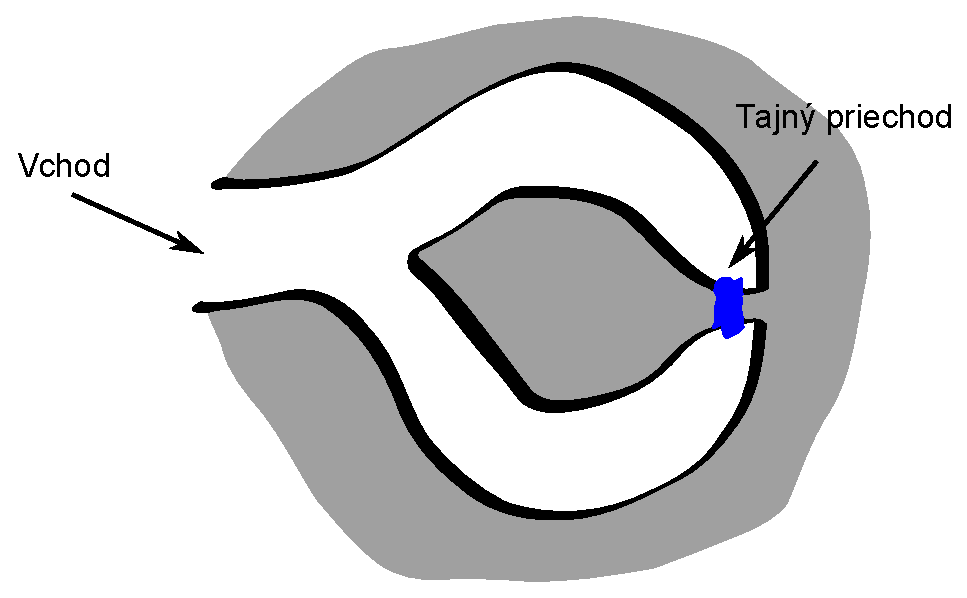
\includegraphics[scale=0.4]{img/x/alibaba}
    
    \label{fig:alibaba}
    \caption{Alibabova jaskyňa}
\end{figure}

Preto sa s filmármi dohodol na nasledujúcom postupe - vôjde do jaskyne
sám. Následne dnu vojde aj filmový štáb a ten zakričí Aladinovi, z
ktorej strany má dôjsť. Ten na demonštráciu znalosti prechádzania cez
steny vyjde zo správnej strany.

Poučenie z príbehu: Môžeme si všimnúť, že Aladin nikomu neprezradí
svoje tajomstvo. Zároveň ale presvedčí štáb o tom, že cez tie steny
chodí, pretože inak by si musel vedieť niekoľkokrát po sebe správne
tipnúť, čo sa mu rozhodnú zakričať, keď dôjdu na rázcestie.
Dôkaz má ale aj ďalšiu vlastnosť - Aladin síce presvedčil štáb, ale
môže presvedčiť aj divákov? Nie. Čo ak bolo napríklad video
"nastrihané" iba na dobré pokusy?

Bezznalostné dokazovacie systémy sú preto také systémy, pri ktorých
dokazovateľ presvedčí overovateľa o svojej pravde bez toho aby mu
prezradil čokoľvek iné. Taktiež, ľubovoľný externý pozorovateľ
komunikácie nemá byť schopný odlíšiť reálny dôkaz od akéhosi
vykonštruovaného.


\todo{zvysok, blackbox simulator}
\todo{ZK pre izomorfizmus}
\todo{preco neizomorfixmus (ako je prezentovany) nie je ZK}
\begin{poznamka}
    Na tomto mieste by sme upozornili čitateľa na fakt, že nami
    prezentovaný algoritmus v predchádzajúcej sekcii na neizomorfizmus grafov
    nie je bezznalostný.
    
    Prečo? Uvažujme falošného verifikátora $V'$,
    ktorý má graf $G$ a vie, že je izomorfný buď s $G_0$ alebo s
    $G_1$. V tomto prípade môže využiť provera $P$ ako orákulum na
    problém izomorfizmu grafov - jednoducho mu pošle $G$, čo je
    validná správa a vráti sa mu index.

    No dobre. A ako súvisí to, že $V'$ vie niečo zistiť s definíciou
    bezznalosti, t.j. s existenciou simulátora? Jednoducho tak, že
    každý polynomiálny simulátor by musel vedieť simulovať komunikáciu
    $P$ s $V'$. Toto ale nemôže vedieť, pretože by sme vedeli v
    polynomiálnom čase riešiť izomorfizmus grafov, čo za predpokladu
    $P\neq NP$ nevieme. Preto dôkaz nie je bezznalostný z definície.
    Záverom teda môžeme usudzovať, že existencia polynomiálneho
    simulátora je naozaj ekvivalentná našej intuícii, čo to znamená
    "bezznalostný".

    Pre záujemcov o bezznalostný algoritmus pre neizomorfizmus grafov
    odporúčame prečítať \cite{nig}, kde je uvedené rozšírenie našeho
    postupu tak, aby $P$ nič neprezradil.
\end{poznamka}

\section{Bit commitment}

Bit commitment schéma je protokol pre dvoch účastníkov, kde sa najprv účastník
zaviaže k nejakému bitu a následne po istom čase ho odhalí.
Formálne to môžeme definovať takto:

\begin{definicia}
Majme dve množiny $X,Y$ a funkciu $f\colon \{0,1\} \times X \to Y$, ktorú vieme
\clqq ľahko\crqq počítať. Od $f$ požadujeme navyše ešte tieto vlastnosti:
\begin{itemize}
\item Zo znalosti $f(b,x)$ je ťažké určiť $b$ - vlastnosť utajenia.
\item Je ťažké nájsť $x, y$ také, že $x \neq y$ a $f(0,x) = f(1,y)$ - vlastnosť záväznosti.
\end{itemize}
Potom bit commitment protokol vyzerá nasledovne:
\begin{enumerate}
\item $A$ zvolí $b \in \{0,1\}$ ku ktorému sa chce zaviazať a $x \inr X$
\item $A \to B$: $y = f(b,x)$ - záväzok
\item $A \to B$: $x$ - odhalenie, môže prísť po istom čase
\item $B$ overí, či $y = f(0,x)$ alebo $y = f(1,x)$
\end{enumerate}
\end{definicia}

Tento protokol môžeme realizovať viacerými spôsobmi. 

\noindent{\bf{Bit commitment pomocou RSA}}

Majme nejakú inštanciu RSA systému, teda trojicu $(n,e,d)$, kde účastník $b$ nepozná súkromný kľúč.
Bit commitment realizujeme nasledovne:
\begin{enumerate}
\item Záväzok: $A$ si zvolí $x \inr \mathbb{Z}_n^*$ a pošle $B$: $y = x^e \pmod n$, v tomto prípade je $b$ najmenej signifikatný bit z $x$
\item Odhalenie: $A$ pošle $x$. $B$ overí, či $x^e \pmod n = y$
\end{enumerate}

Vlastnosť utajenia je dodržaná, keďže možnosť zistiť $b$ je ekvivalentná rozbitiu RSA schémy.
Vlastnosť záväznosti je tiež dodržaná, keďže k jednému $y$ existuje iba jedno $x$. V tomto prípade ide o nepodmienenú bezpečnosť.

\todo{realizacia cez diskretny logaritmus}
\todo{IDS pre ham cycle pomocou BC}



\input{xkrypto1/ot.tex}
\section{Bezpecny vypocet viacerych ucastnikov}

\todo{porovnavanie veku}
\todo{\url{http://www.derkeiler.com/Newsgroups/sci.crypt/2006-10/msg00665.html}}

\todo{bezpecny vypocet funkcie}



\chapter{Krypto II}
\label{chapter:krypto2}
\input{tex/11abs.tex}
\subsection{PSS - Probabilistic signature scheme}

PSS je dokázateľne bezpečná (za istých predpokladov) schéma na
digitálne podpisy. Navrhli ju páni Mihir Bellare a Philip Rogaway
v \cite{pss}. Celá schéma je vlastne akýmsi znáhodnením hashovania - k
správe sa pridá náhodný reťazec dĺžky $k_0$ a hash sa počíta až
potom. Samozrejme, pri overovaní hashu treba nejakým spôsobom
vyriešiť, aby sme sa dozvedeli použitý náhodný reťazec. Ako sa ukáže
neskôr, toto nie je až taký veľký problém ak použijeme ďalšiu
hashovaciu funkciu.

PSS má oproti doteraz spomínaným schémam jednu veľkú výhodu - pri
dôkaze jej bezpečnosti sa ukáže ``tesná'' hranica. T.j., možnosť
prelomiť PSS s pravdepodobnosťou $\eps$ priamo umožňuje lámanie RSA s
rovnakou pravdepodobnosťou.


\subsubsection{RSA-PSS}

Podpisová schéma $PSS[k_0,k_1]=(GenPSS,SignPSS,VerifyPSS)$ je
parametrizovaná dvoma hodnotami $k_0, k_1$.
Generovanie kľúča $k$ je presne rovnaké ako v $GenRSA-FDH$.

Pri podpisovaní bude náš algoritmus používať 2 hashovacie funkcie.
Prvú si označíme $h$ a nazveme ju kompresor, pretože 
$h:\{0,1\}^* \rightarrow \{0,1\}^{k_1}$.
Druhá funkcia bude $g$ (nazvaná aj generátor), pričom
$g:\{0,1\}^{k_1} \rightarrow \{0,1\}^{k-k_1-1}$.

Ešte si označíme $g_1$, resp. $g_2$ ako funkciu, ktorá vracia
prvých $k_0$ (resp. zvyšných $k-k_0-k_1-1$) bitov funkcie $g$.

Na obrázku \todo{} je schematicky naznačený postup podpisovania
podľa pseudokódu \ref{proc:signpss}

% {{{ proc SignPSS
\begin{procedure}
    \caption{SignPSS($m$)}
    \label{proc:signpss}
    $r \inr \{0,1\}^{k_0}$\;
    $w \assign h(M \concat r)$\;
    $r^* \assign g_1(w) \xor r$\;
    $y \assign 0 \concat w \concat r^* \concat g_2(w)$\;
    \Return $y^d \bmod N$\;
\end{procedure}
%% }}}

Môžeme si všimnúť, že náhodný reťazec $r$ sme neuviedli v
``otvorenom'' tvare, ale zviazali sme ho funkciou $g_1$. Intuitívne,
toto nám umožní zaručiť jeho integritu a zároveň máme možnosť ho
zrekonštruovať.

Overovanie podpisu je popísané v pseudokóde \ref{proc:verifypss}

%%% {{{ proc VerifyPSS
\begin{procedure}
    \caption{VerifyPSS($m$,$x$)}
    \label{proc:verifypss}
    $y \assign x^e \bmod N$\;
    rozdeľ $y$ na $b \concat w \concat r^* \concat \gamma$\;
    $r \assign r^* \xor g_1(w)$\;
    \eIf{$(b \ne 0) \vee (g_2(w) \ne \gamma) 
            \vee (h(m \concat r) \ne w)$}
    {% then
        \Return reject\;
    }{% else
        \Return accept\;
    }
\end{procedure}
%%% }}}

\todo{nejake omacky okolo funkcnosti a preco je  to zhruba tak
spravene}

\subsubsection{Dôkaz bezpečnosti}
\todo{dokaz bezpecnosti - tesna redukcia}

\input{tex/3factor.tex}
\input{tex/4dlog.tex}
\input{tex/5hash.tex}
\section{Jednorázové & fail-stop podpisové schémy}

Jednorázové podpisové schémy, ako už ich názov napovedá, slúžia na
podpísanie práve jednej správy. Ich bezpečnosť je v prípade viacnásobného
podpisovania ohrozená. Načo sú nám teda takéto podpisové schémy? Zatiaľ to
vyzerá tak, že sú ia menej výhodné. Existujú však dôvody, prečo sa zaoberať
aj takýmito zjavne ``okrátenými'' podpisovými schémami.

Ich hlavná výhoda bude spočívať v jednoduchších predpokladoch pri dôkaze
bezpečnosti. Kým pri bežných podpisových schémach sme stavali na
tažkosti istých matematických problémov (RSA, dlog, Diffie-Hellman),
pri jednorázových schémach nám bude stačiť napríklad jednosmernosť
hashovacej funkcie.\footnote{Už aj toto je pomerne náročný predpoklad,
    keďže nevieme povedať veľa o existencii one-way funkcií}
Druhou výhodou môže byť rýchlosť - zrejme je jednoduchšie hashovať hodnoty
ako napríklad umocňovať.
Treťou výhodou (i keď skôr teoretickou) je možnosť odolať kvantovým
výpočtom - pre väčsinu používaných ťažkých problémov sú známe kvantové
algoritmy, ktoré ich efektívne počítajú. Pre invertovanie hashovacích
funkcií ale takéto algoritmy nie sú známe.

Otázka teda môže znieť, že či jednorázovosť je až taká obmedzujúca
vlastnosť. Môžeme napríklad uvažovať komunikáciu s bankou a podpisovanie
prevodných príkazov. Je jednoducho predstaviteľné, že povedzme za mesiac
bežný človek nespraví viac ako povedzme 5 príkazov. Preto môžeme použiť
niečo ako pohľad z opačnej strany - namiesto toho, aby sme navrhovali
podpisové schémy na polynomiálny počet podpísaných správ,
môžeme sa snažiť navrhnúť schémy na jednorázové podpisy a tie potom
rozšíriť nejakým spôsobom pre viac správ.

Jednorázovú podpisovou schému formálne definujeme veľmi podobne ako bežné
podpisové schémy

\begin{definicia}[Jednorázová podpisová schéma]
    je trojica algoritmov 
    $\langle Gen, Sign_{sk}, Verify_{pk} \rangle$ kde
    $Gen(1^k) \implies \langle pk, sk \rangle$ je generátor kľúčov,
    $Sign_{sk}(m) \implies \sigma$ je podpisovací algoritmus a
    $Verify_{pk}(m,\sigma) \implies \{0,1\}$ je overovací algoritmus.
\end{definicia}

Pojem bezpečnosti takejto schémy si upravíme na jednu správu.
\begin{definicia}[Bezpečnosť]
    Uvažujme útočníka ako PPT algoritmus, ktorý má navyše k dispozícii
    orákulum $Sig_{sk}$. Útočník sa môže raz opýtať orákula na podpis
    $\sigma$ správy $m$ a jeho cieľom je zostrojiť
    správu $m' \ne m$ a k nej platný podpis $\sigma'$.
    Budeme hovoriť, že schéma je bezpečná ak pravdepodobnosť,
    že ľubovoľný útočník uspeje (t.j. nájde $(m',\sigma')$), je zanedbateľná.
\end{definicia}

\subsection{\fixme{spelling}Lampartova schéma}


\section{Inkrementálne hašovanie}

\subsubsection{Motivácia}

Predstavme si, že máme dlhý dokument (súbor, disk),
označme ho $m$ a chceme si uchovávať jeho hash. Pri klasickom riešení
by sme museli prejsť celý dokument a spočítať jeho 
hash $H(m)$. Následne keď urobíme čo i len najmenšiu
zmenu, tak na to, aby sme získali novú hash musíme opäť
prejsť celý súbor. Toto je náročné na systémové prostriedky.

\subsection{Triviálne riešenia}

Môžeme náš dokument rozdeliť na časti (disk na sektory)
a uchovávať hash každej časti osobitne. V prípade, keď
$m = m_1 m_2 \dots m_k$, tak hash bude 
$H(m) = <h(m_1), h(m_2), \dots, h(m_k)>$.
Toto riešenie má ale oveľa dlhšiu hash.

Iné riešenie je použiť Merkleho stromy. Tak si ale preto, aby
sme mali rýchly update hashe musíme pamätať zloženie celého stromu, čo tiež nie je potešujúce.


\subsection{Lepšie riešenia}

Zoberme konečnú komutatívnu grupu $(G, \odot)$ (napr. $(2^n, XOR)$).
Následne predpokladajme, že máme hašovaciu funkciu s oborom hodnôť $G$.
Rozdeľme dokument na $k$ blokov $m = x_1 x_2 \dots x_k$ Naša hash bude 
$H(m) = \displaystyle\bigodot_{j=1}^k h(i, x_i)$. 
Pokiaľ sa blok $x_i$ zmení na $x_i^{'}$, tak nová hash bude:
$$H(m^{'}) = H(m) \odot h(i, x_i)^{-1} \odot h(i, x_i^{'})$$

\subsubsection{Súvislosť s problémom vyvažovania}

Dá sa ukázať, že nájsť kolíziu pre incrementálnu hašovaciu
funkciu používajúcu grupu $G$ je aspoň tak ťažké ako riešiť
problém vyvažovania (ktorého obťiažnosť závisí hlavne od grupy 
$G$).

\begin{definicia}
Máme zadanú grupu $(G, \odot)$ a postupnosť $a_1, a_2, \dots, a_n$. Našou úlohou
je nájsť čísla $w_1, w_2, \dots, w_n \in \{-1, 0, 1\}$, kde aspoň jedno z nich
je nenulové a platí $a_1^{w_1} \odot a_2^{w_2} \odot \dots \odot a_n^{w_n}$.
Tomuto problému hovoríme problém vyvažovania.
\end{definicia}

\begin{poznamka}
Pokiaľ je grupa $G$ komutatívna, tak vlastne hľadáme dve neprázdne disjuktné podmnožiny
$I, J \subseteq \{1, 2, \dots, n\}$, kde platí $\bigodot_{i\in I} a_i = \bigodot_{j \in J} a_j$.
\end{poznamka}

\begin{lema}
Ak vieme v grupe $(G, \odot)$ hľadať kolízie pre inkrementálne hašovacie
funkcie, tak vieme rovnako efektívne riešiť problém vyvažovania.
\end{lema}

\begin{dokaz}
Majme orákulum $A$, ktoré hľadá kolíziu pre inkrementálnu hašovaciu
funkciu nad grupou $(G, \odot)$. Toto orákulum nám položí $q$ otázok
typu aká je hodnota $h(i, x_i)$. Na tieto otázky mu odpovieme postupne $a_1, a_2, \dots, a_q$.
Orákulum podá odpoveď $H(x) = H(y)$, čo je vlastne $\bigodot_{i \in I} a_i = \bigodot_{j \in J} a_j$.
(Keďže predpokladáme, že funkcia $h$ sa správa ako náhodné orákulum, tak sa na všetky zložky
$x$ a $y$ musí $A$ opýtať.)
\end{dokaz}

\subsection{XOR-hash}

Najprv si ukážeme tzv. XOR-HASH.
Predpokladajme, že $h\colon \{0,1\}^l \to \{0,1\}^n$.
Hash bude daná vzorcom:
$H(m) = \displaystyle\bigoplus_{j=1}^k h(i, x_i)$.

Ukážeme, že aj v prípade, že $h$ je kvalitná hašovacia funkcia
(správa sa ako náhodné orákulum) vieme XOR-HASH invertovať.

Na vstupe majme $z \in \{0,1\}^n$. Najprv si pripravíme
2 náhodné dokumenty $x^0 = x_1^0 x_2^0 \dots x_k^0$ a 
$x_1 = x_1^1 x_2^1 \dots x_k^1$. Spočítame si hashe ich častí:
$a_i^b = h(i, x_i^b)$. 
Teraz chceme nájsť $y = y_1 y_2 \dots y_k$, kde $y_1 \in \{0,1\}$,
také, že $z = a_1^{y_1} \oplus a_2^{y_2} \oplus \dots \oplus a_k^{y_k}$
(teda $H(x_1^{y_1} x_2^{y_2} \dots x_k^{y_k}) = z$).
Táto rovnica sa dá napísať aj ako:
$$z = a_1^0 (1 - y_1) \oplus a_1^1 y_1 \oplus \dots \oplus a_k^0 (1 - y_k) \oplus a_k^1 y_k$$

Keďže $z$ má $n$ bitov a všetky tieto bity sa počítajú nezávisle od ostatných vieme
zostaviť $n$ rovníc nad $Z_2$. A máme $k$ neznámych. Keďže v praktických
aplikáciách je $k > n$ dostaneme skoro vždy riešenie.

\todo{sanca na najdenie riesenia}

\subsection{Ad-hash}

Tento krát spravíme iteratívnu hash v grupe $(Z_m, +)$.
Tu sa dá ukázať, že problém vyvažovania pre $(Z_m, +)$
je ťažký. 

V praxi sa používajú napr. tieto 2 konštrukcie:

NASD konštrukcia:
$$H(x) = \displaystyle\sum_{i=1}^k h(i, x_i) \bmod 2^{256}$$

DCIHF konštrukcia:
$$H(x) = \displaystyle\sum_{i=1}^{k-1} \textrm{SHA-1}(x_i, x_{i+1}) \bmod 2^{160}+1$$

\todo{zovseobecneny birthday attack}


\section{Identity based crypto}

Asymetrické kryptovacie systémy, ktoré veľmi dobre poznáme, vyžadujú,
aby si každý vygeneroval vlastnú inštanciu danej schémy. Problém pri
takomto riešení je distribúcia verejného kľúča. Ak nemám dostatočne
dôveryhodný kanál na distribúciu môjho verejného kľúča, útočník si
môže pripraviť vlastný kľúč a presvedčiť obeť o tom, že je to môj
kľúč. Navyše, existujú isté ťažkosti s udržiavaním verejných kľúčov a
limity sú aj v chápanlivosti ľudí o potrebe bezpečného kanálu pri
distribúcii.
Isté riešenie tohoto problému,
ktoré sa ujalo najmä pri webových aplikáciach sú certifikáty --
kľúč sa podpíše dôveryhodnou autoritou a každý si môže
overiť, že po kanáli dostal správny kľúč. V tejto kapitole sa budeme
venovať alternatívnemu riešeniu -- verejným kľúčom bude priamo moja
identita.

Ako si to teda môžeme predstaviť? Nebudeme generovať inštanciu schémy,
ale uvažujme rovno, že mojím kľúčom bude priamo moja identifikácia -
či už email, OpenID konto a pod.

Na pomoc si ale budeme musieť prizvať dôveryhodnú tretiu stranu $T$.
Táto strana bude mať 2 kľúče master public key $M_{pk}$ a master
secret key $M_{sk}$. Túto tretiu stranu budeme potrebovať, aby nám
vygenerovala náš súkromný kľúč k môjmu verejnému kľúču (kontu).
Formálne, toto generovanie si môžeme popísať ako algoritmus, ktorý
užívateľovi $U$ priradí na záklede jeho identity $ID_U$ jeho súkromný
kľúč $U_{sk} = Extract(M_{sk}, ID_U)$. Samozrejme, kľúč ešte treba
dôveryhodne doručiť, toto ale nebudeme riešiť.

Potom môžeme šifrovať a dešifrovať nasledovne:
$c=E(m,ID_U,M_{pk})$ a opačne $m = D(c, U_{sk}, M_{pk})$, pričom
samozrejme požadujeme
$\forall ID_U \forall m: D(E(m, ID_U, M_{pk}), Extract(M_{sk},ID_U),
M_{pk})=m$.

Takáto schéma má ale výraznú bezpečnostnú slabinu - kompromitácia
$M_{sk}$ je fatálna. Je teda otázne, do akej miery môžeme dôverovať
zabezpečeniu dôveryhodnej strany. Napriek tomuto problému si ukážeme,
ako môže taká schéma fungovať.

\subsection{Coksova schéma (2001)}
\todo{cela schema}


%\backmatter fixme: preco to tu nefunguje? asi chyba nejaky package
\listoffigures
\listoftables

\bibliographystyle{alpha}
\bibliography{literatura}



\end{document}
